\documentclass{beamer}
\usepackage{listings}
\lstset{
%language=C,
frame=single, 
breaklines=true,
columns=fullflexible
}
\usepackage{blkarray}
\usepackage{subcaption}
\usepackage{url}
\usepackage{tikz}
\usepackage{tkz-euclide} % loads  TikZ and tkz-base
%\usetkzobj{all}
\usetikzlibrary{calc,math}
\usepackage{float}
\newcommand\norm[1]{\left\lVert#1\right\rVert}
\renewcommand{\vec}[1]{\mathbf{#1}}
\usepackage[export]{adjustbox}
\usepackage[utf8]{inputenc}
\usepackage{amsmath}
\usepackage{tikz}
\usetikzlibrary{automata, positioning}
\usetheme{Boadilla}
\providecommand{\sbrak}[1]{\ensuremath{{}\left[#1\right]}}
\providecommand{\lsbrak}[1]{\ensuremath{{}\left[#1\right.}}
\providecommand{\rsbrak}[1]{\ensuremath{{}\left.#1\right]}}
\providecommand{\pr}[1]{\ensuremath{\Pr\left(#1\right)}}
\providecommand{\brak}[1]{\ensuremath{\left(#1\right)}}
\providecommand{\lbrak}[1]{\ensuremath{\left(#1\right.}}
\providecommand{\rbrak}[1]{\ensuremath{\left.#1\right)}}
\providecommand{\cbrak}[1]{\ensuremath{\left\{#1\right\}}}
\providecommand{\lcbrak}[1]{\ensuremath{\left\{#1\right.}}
\providecommand{\rcbrak}[1]{\ensuremath{\left.#1\right\}}}

\title{CSIR-UGC NET-June 2013-Problem(72)}
\author{Yashas Tadikamalla}
\date{AI20BTECH11027}
\begin{document}

\begin{frame}
\titlepage
\end{frame}

\begin{frame}
\frametitle{}
\begin{block}{Convergence in Probability}
A sequence of random variables $X_{1},X_{2},X_{3},\dots$ converges in probability to a random variable $X$, if
\begin{align}
    \label{eq:p}
    \displaystyle\lim_{n\to\infty}\pr{|X_{n}-X|\geq\epsilon}=0,\forall\epsilon>0
\end{align}
Notation : $X_{n}\xrightarrow[]{p}X$
\end{block}
\begin{block}{Convergence in Distribution}
A sequence of random variables $X_{1},X_{2},X_{3},\dots$ converges in distribution to a random variable $X$, if
\begin{align}
    \label{eq:d}
    \displaystyle\lim_{n\to\infty}F_{X_{n}}(x)=F_{X}(x)
\end{align}
for all $x$ at which $F_{X}(x)$ is continuous.\\
Notation : $X_{n}\xrightarrow[]{d}X$
\end{block}
\end{frame}

\begin{frame}
\frametitle{}
\begin{block}{Random Sampling}
A collection of random variables $X_{1},X_{2},\dots,X_{n}$ is said to be a random sample of size $n$ if they are independent and identically distributed, i.e,
\begin{enumerate}
    \item $X_{1},X_{2},\dots,X_{n}$ are independent random variables
    \item They have the same distribution (Let us denote it by $F_{X}(x)$), i.e,
    \begin{align}
        F_{X}(x)=F_{X_{1}}(x)=F_{X_{2}}(x)=\dots=F_{X_{n}}(x),\forall x\in \mathbb{R}
    \end{align}
\end{enumerate}
\end{block}
\begin{block}{Order Statistics}
Given a random sample $X_{1},X_{2},\dots,X_{n}$, the sequence $X_{(1)},X_{(2)},\dots,X_{(n)}$ is called the order statistics of it. Here,
\begin{align}
    &X_{(1)}=\min\brak{X_{1},X_{2},\dots,X_{n}}\\
    &X_{(2)}=\text{the }2^{nd}\text{ smallest of }X_{1},X_{2},\dots,X_{n}\\
    &\vdots\\
    &X_{(n)}=\max\brak{X_{1},X_{2},\dots,X_{n}}
\end{align}
\end{block}
\end{frame}

\begin{frame}
\frametitle{}
\begin{block}{Distribution of the maximum}
Let's calculate the CDF, PDF of $X_{(n)}$
\begin{align}
   F_{X_{(n)}}(x)&=\pr{X_{(n)}\leq x}=\pr{X_{1}\leq x,X_{2}\leq x,\dots,X_{n}\leq x}\\
   &=\pr{X_{1}\leq x}\pr{X_{2}\leq x}\dots\pr{X_{n}\leq x}\brak{\because \text{independence}}\\
   \label{eq:F}
   &=\sbrak{\pr{X_{1}\leq x}}^{n}\brak{\because \text{identical distribution}}=\sbrak{F_{X}(x)}^{n}
\end{align}
\begin{align}
   f_{X_{(n)}}(x)&=\dfrac{d}{dx}\brak{F_{X_{(n)}}(x)}=\dfrac{d}{dx}\brak{\sbrak{F_{X}(x)}^{n}}\\
   &=n\brak{\sbrak{F_{X}(x)}^{n-1}}\dfrac{d}{dx}\brak{F_{X}(x)}\\
   \label{eq:f}
   &=n\sbrak{F_{X}(x)}^{n-1}f_{X}(x)\brak{\because\dfrac{d}{dx}\brak{F_{X}(x)}=f_{X}(x)}
\end{align}
\end{block}
\end{frame}

\begin{frame}
\frametitle{}
\begin{block}{Uniform Distribution}
A continuous random variable $X$ is said to have a Uniform Distribution over the interval (a,b), shown as $X\sim Uniform(a,b)$, if,
\begin{align}
        f_{X}(x)=\begin{cases}
	\frac{1}{b-a}, & a< x<b \\~\\[-1em]
	0, & otherwise
	\end{cases},F_{X}(x)=\begin{cases}
	x, & a< x<b \\~\\[-1em]
	1, & x\geq b\\~\\[-1em]
	0, & otherwise
	\end{cases} 
\end{align}
\end{block}
\begin{block}{Exponential Distribution}
A continuous random variable $X$ is said to have an exponential distribution with parameter $\lambda>0$, shown as $X\sim Exponential(\lambda)$, if 
\begin{align}
        f_{X}(x)=\begin{cases}
	\lambda e^{-\lambda x}, & x>0\\~\\[-1em]
	0, & otherwise
	\end{cases},F_{X}(x)=\begin{cases}
	1-e^{-\lambda x}, & x>0 \\~\\[-1em]
	0, & otherwise
	\end{cases} 
\end{align}
\end{block}
\end{frame}

\begin{frame}
\frametitle{Question}
\begin{block}{CSIR-UGC NET-June 2013-Problem(72)}
Let $X_{1},X_{2},\dots$ be independent and identically distributed random variables each following a uniform distribution on (0,1). Denote $T_{n}=\max\brak{ X_{1},X_{2},\dots,X_{n}}$. Then, which of the following statements are true?
\begin{enumerate}
    \item $T_{n}$ converges to 1 in probability.
    \item $n(1-T_{n})$ converges in distribution.
    \item $n^{2}(1-T_{n})$ converges in distribution.
    \item $\sqrt{n}(1-T_{n})$ converges to 0 in probability.
\end{enumerate}
\end{block}
\end{frame}

\begin{frame}
\frametitle{Solution}
Given, $X_{1},X_{2},X_{3},\dots$ are independent and identically distributed random variables each following a uniform distribution on (0,1). Let us denote their PDF, CDF by $f_{X}(x),F_{X}(x)$ respectively. Then,
\begin{align}
    f_{X}(x)=\begin{cases}
	1, & 0< x<1 \\~\\[-1em]
	0, & otherwise
	\end{cases} 
\end{align}
\begin{align}
	F_{X}(x)=\begin{cases}
	x, & 0< x<1 \\~\\[-1em]
	1, & x\geq 1\\~\\[-1em]
	0, & otherwise
	\end{cases} 
\end{align}
\end{frame}

\begin{frame}
\frametitle{Solution Contd.}
As $T_{n}=\max\brak{X_{1},X_{2},\dots,X_{n}}=X_{(n)}$, from \eqref{eq:f}
\begin{align}
    f_{T_{n}}(x)=\begin{cases}
	nx^{n-1}, & 0< x<1 \\~\\[-1em]
	0, & otherwise
	\end{cases} 
\end{align}
Also, from \eqref{eq:F}
\begin{align}
	F_{T_{n}}(x)=\begin{cases}
	x^{n}, & 0< x<1 \\~\\[-1em]
	1, & x\geq 1\\~\\[-1em]
	0, & otherwise
	\end{cases} 
\end{align}
\end{frame}

\begin{frame}
\frametitle{Note}
\begin{block}{}
Let $X$ be a continuous random variable. If $Y=aX+b$ and $a<0$, then
\begin{align}
\label{eq:form}
    F_{Y}(y)=1-F_{X}\brak{\dfrac{y-b}{a}}
\end{align}
\end{block}
\begin{block}{Proof}
    \begin{align}
        F_{Y}(y)&=\pr{Y\leq y}=\pr{aX+b \leq y}\\
        &=\pr{X \geq\brak{\dfrac{y-b}{a}}}\brak{\because a<0}\\
        &=1-\pr{X \leq\brak{\dfrac{y-b}{a}}}+\pr{X =\brak{\dfrac{y-b}{a}}}\\
        &=1-F_{X}\brak{\dfrac{y-b}{a}}+0=1-F_{X}\brak{\dfrac{y-b}{a}}
    \end{align}
\end{block}
\end{frame}

\begin{frame}
\frametitle{Option 1}
Consider the sequence of random variables $X_{1},X_{2},X_{3},\dots$, such that $X_{n}=T_{n}$. From \eqref{eq:p}, we need to evaluate $\displaystyle\lim_{n\to\infty}\pr{|T_{n}-1|\geq\epsilon},\forall\epsilon>0$
\begin{align}
    &\displaystyle\lim_{n\to\infty}\pr{|T_{n}-1|\geq\epsilon}=\displaystyle\lim_{n\to\infty}\pr{1-T_{n}\geq\epsilon}\\
    &=\displaystyle\lim_{n\to\infty}\pr{T_{n}\leq1-\epsilon}=\displaystyle\lim_{n\to\infty}F_{T_{n}}(1-\epsilon)\\
    &F_{T_{n}}(1-\epsilon)=\begin{cases}
	(1-\epsilon)^{n}, & 0< \epsilon<1 \\~\\[-1em]
	0, & \epsilon\geq 1
	\end{cases}\\
    &\because\displaystyle\lim_{n\to\infty}(1-\epsilon)^{n}=0 \text{ for } 0< \epsilon<1\\
    &\therefore \displaystyle\lim_{n\to\infty}\pr{|T_{n}-1|\geq\epsilon}=0,\forall\epsilon>0
\end{align}
$\therefore T_{n}$ converges to 1 in probability.
\end{frame}

\begin{frame}
\frametitle{Option 2}
Consider the sequence of random variables $X_{1},X_{2},X_{3},\dots$, such that $X_{n}=n(1-T_{n})$. From \eqref{eq:d}, we need to evaluate $\displaystyle\lim_{n\to\infty}F_{n(1-T_{n})}(x)$. Substituting $a=-n,b=n$ in \eqref{eq:form},
\begin{align}
    &F_{n(1-T_{n})}(x)=1-F_{T_{n}}\brak{1-\dfrac{x}{n}}\\
    &F_{T_{n}}\brak{1-\dfrac{x}{n}}=\begin{cases}
	\brak{1-\dfrac{x}{n}}^{n}, & 0< x<n \\~\\[-1em]
	1, & x\leq 0\\~\\[-1em]
	0, & x\geq n
	\end{cases} \\
    &\because\displaystyle\lim_{n\to\infty}\brak{1-\dfrac{x}{n}}^{n}=e^{-x}
\end{align}
\end{frame}

\begin{frame}
\frametitle{Option 2 Contd.}
\begin{align}
&\therefore\displaystyle\lim_{n\to\infty} F_{T_{n}}\brak{1-\dfrac{x}{n}}=\begin{cases}
	e^{-x}, & x>0 \\~\\[-1em]
	1, & x\leq 0
	\end{cases} \\
&\because\displaystyle\lim_{n\to\infty}F_{n(1-T_{n})}(x)=1-\displaystyle\lim_{n\to\infty} F_{T_{n}}\brak{1-\dfrac{x}{n}}\\
\label{eq:cdf1}
    &\therefore\displaystyle\lim_{n\to\infty} F_{n(1-T_{n})}(x)=\begin{cases}
	1-e^{-x}, & x>0 \\~\\[-1em]
	0, & x\leq 0
	\end{cases} 
\end{align}
$\because$ The CDF in \eqref{eq:cdf1} represents an exponential distribution with $\lambda=1$\\
$\therefore n(1-T_{n})$ converges in distribution to the random variable $X\sim Exponential(1)$.
\end{frame}

\begin{frame}
\frametitle{Option 2 Contd.}
\begin{figure}[h!]
\centering
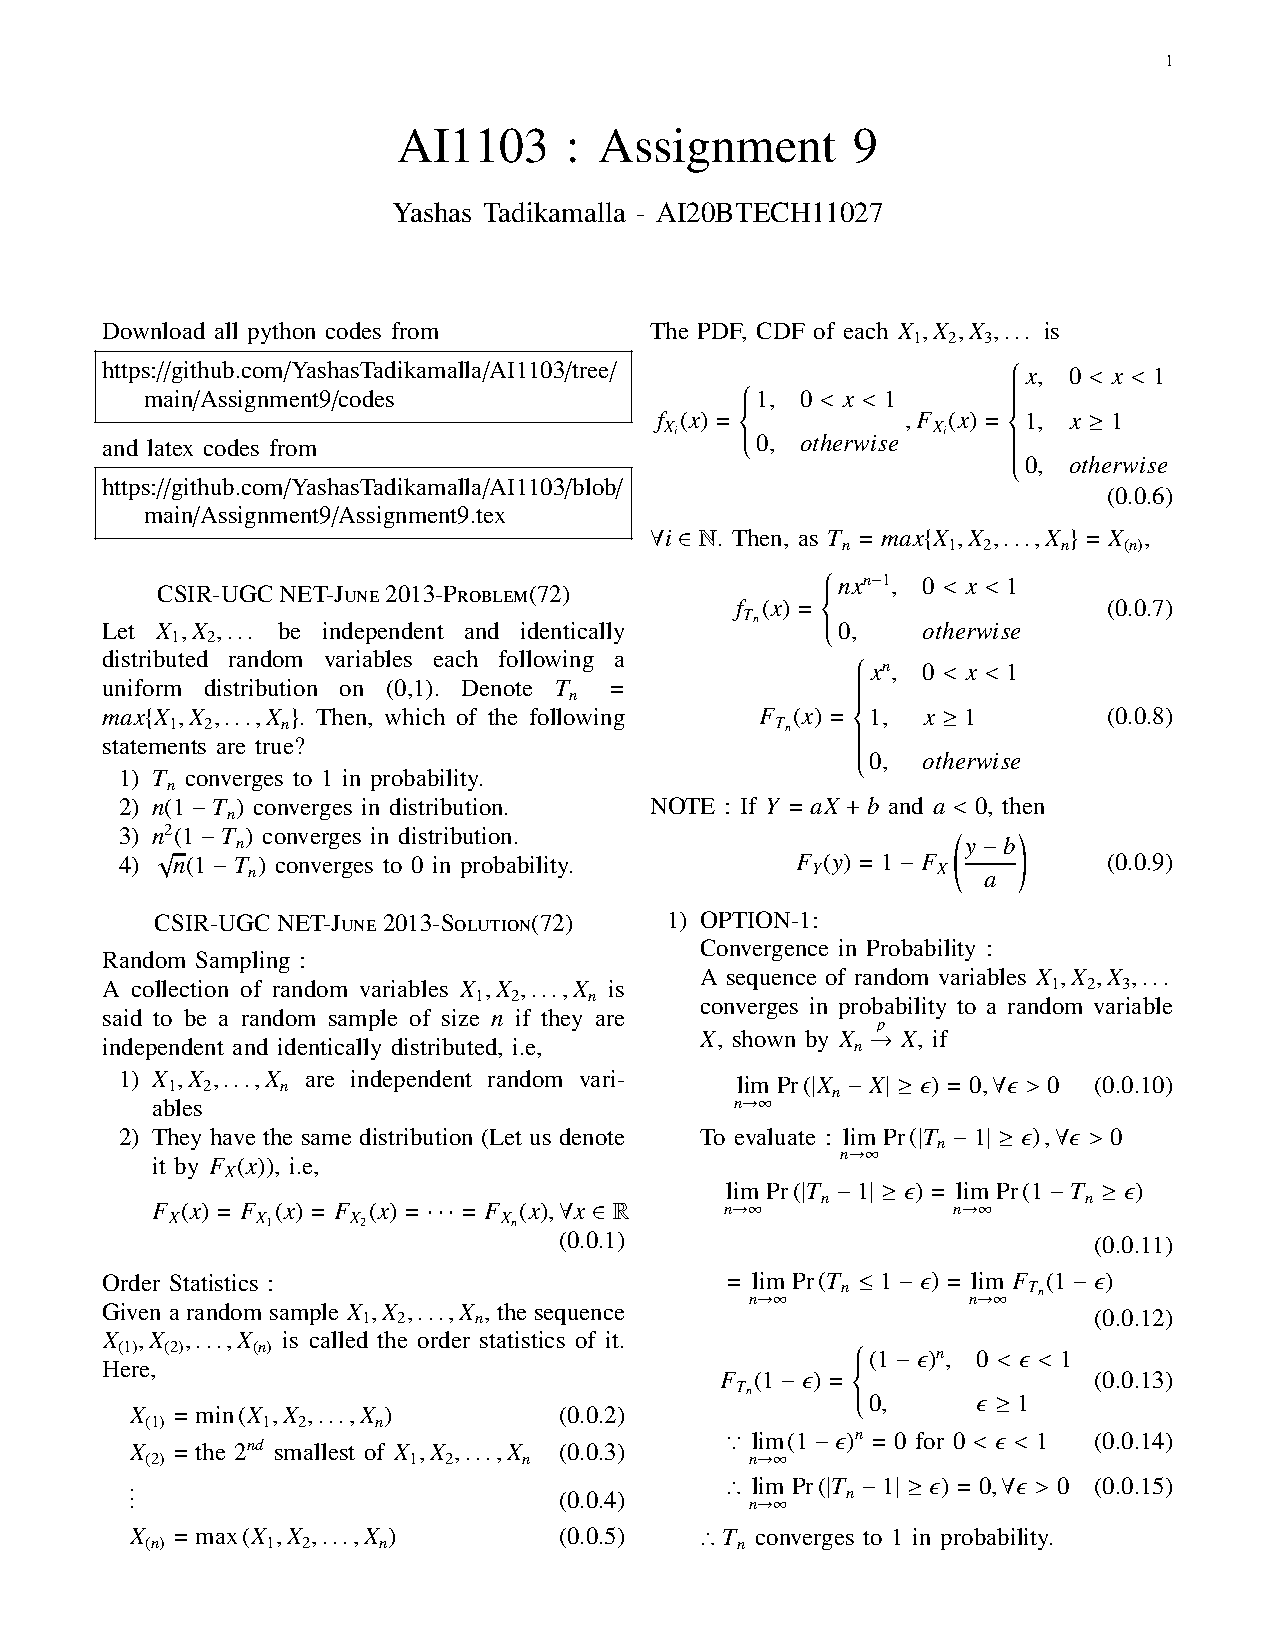
\includegraphics[width=0.75\linewidth]{Assignment9}
\caption{Plot for the CDF defined in \eqref{eq:cdf1}  }
\label{plot}
\end{figure}
\end{frame}

\begin{frame}
\frametitle{Option 3}
Consider the sequence of random variables $X_{1},X_{2},X_{3},\dots$, such that $X_{n}=n^{2}(1-T_{n})$. From \eqref{eq:d}, we need to evaluate $\displaystyle\lim_{n\to\infty}F_{n^{2}(1-T_{n})}(x)$. Substituting $a=-n^{2},b=n^{2}$ in \eqref{eq:form},
\begin{align}
    &F_{n^{2}(1-T_{n})}(x)=1-F_{T_{n}}\brak{1-\dfrac{x}{n^{2}}}\\
    &F_{T_{n}}\brak{1-\dfrac{x}{n^{2}}}=\begin{cases}
	\brak{1-\dfrac{x}{n^{2}}}^{n}, & 0< x<n^{2} \\~\\[-1em]
	1, & x\leq 0\\~\\[-1em]
	0, & x\geq n^{2}
	\end{cases} \\
    &\because\displaystyle\lim_{n\to\infty}\brak{1-\dfrac{x}{n^{2}}}^{n}=1
\end{align}
\end{frame}

\begin{frame}
\frametitle{Option 3 Contd.}
\begin{align}
&\therefore\displaystyle\lim_{n\to\infty} F_{T_{n}}\brak{1-\dfrac{x}{n^{2}}}=\begin{cases}
	1, & x>0 \\~\\[-1em]
	1, & x\leq 0
	\end{cases} \\
&\because\displaystyle\lim_{n\to\infty}F_{n^{2}(1-T_{n})}(x)=1-\displaystyle\lim_{n\to\infty} F_{T_{n}}\brak{1-\dfrac{x}{n^{2}}}\\
\label{eq:cdf2}
    &\therefore\displaystyle\lim_{n\to\infty} F_{n^{2}(1-T_{n})}(x)=\begin{cases}
	0, & x>0 \\~\\[-1em]
	0, & x\leq 0
	\end{cases} 
\end{align}
$\because$ The CDF in \eqref{eq:cdf2} is not valid,\\
$\therefore n^{2}(1-T_{n})$ does not converge in distribution.
\end{frame}

\begin{frame}
\frametitle{Option 4}
Consider the sequence of random variables $X_{1},X_{2},X_{3},\dots$, such that $X_{n}=\sqrt{n}(1-T_{n})$. From \eqref{eq:p}, we need to evaluate $\displaystyle\lim_{n\to\infty}\pr{|\sqrt{n}(1-T_{n})-0|\geq\epsilon},\forall\epsilon>0$
\begin{align}
    &\displaystyle\lim_{n\to\infty}\pr{|\sqrt{n}(1-T_{n})-0|\geq\epsilon}=\displaystyle\lim_{n\to\infty}\pr{1-T_{n}\geq\dfrac{\epsilon}{\sqrt{n}}}\\&=\displaystyle\lim_{n\to\infty}\pr{T_{n}\leq1-\dfrac{\epsilon}{\sqrt{n}}}=\displaystyle\lim_{n\to\infty}F_{T_{n}}\brak{ 1-\dfrac{\epsilon}{\sqrt{n}}}\\
    &F_{T_{n}}\brak{1-\dfrac{\epsilon}{\sqrt{n}}}=\begin{cases}
	\brak{1-\dfrac{\epsilon}{\sqrt{n}}}^{n}, & 0< \epsilon< \sqrt{n}\\~\\[-1em]
	0, & \epsilon\geq \sqrt{n}
	\end{cases}
\end{align}
\end{frame}
    
\begin{frame}
\frametitle{Option 4 Contd.}
\begin{align}
&\because\displaystyle\lim_{n\to\infty}\brak{1-\dfrac{\epsilon}{\sqrt{n}}}^{n}=0 \text{ for } 0< \epsilon<\sqrt{n}\\
    &\therefore \displaystyle\lim_{n\to\infty}\pr{|\sqrt{n}(1-T_{n})-0|\geq\epsilon}=0,\forall\epsilon>0
\end{align}
$\therefore\sqrt{n}(1-T_{n})$ converges to 0 in probability.
\end{frame}

\begin{frame}
\frametitle{Solution Contd.}
Therefore, options 1), 2), 4) are correct.
\end{frame}


\end{document}
